%
%  Chad Conrad
%
\documentclass[12pt,fullpage]{article}
\usepackage{fullpage}
\usepackage{psfrag}                                          % LaTeX graphics tool
\usepackage{pslatex}                                         % avoids the default cmr font
\usepackage{graphicx}                                        % graphics package 
\usepackage{epsfig}                                          % figures
\usepackage{hyperref}
\usepackage{color}

\begin{document}

\noindent
{\bf Chi-square distribution}
(from \color{blue}\url{http://www.math.wm.edu/~leemis/chart/UDR/UDR.html}\color{black})

\noindent
The shorthand $X \sim {\rm \chi^{2}}(n)$ is used to indicate that the
random variable $X$ has the chi-square distribution with positive
real-valued parameter $n$, which is known
as the degrees of freedom.
In most applications, $n$ is a positive integer.
A chi-square random variable $X$ with $n$ degrees of freedom has
probability density function 
$$
f(x) = \frac{x^{n/2-1}e^{-x/2}}{2^{n/2}\kern 0.08 em \Gamma(n/2)} \qquad \qquad x > 0,
$$
for $n = 1, \, 2, \,  \ldots \,$. 
The chi-square distribution is used for inference concerning
observations drawn from an exponential population and in
determining the critical values for the chi-square goodness-of-fit test.
The probability density function with $n=1,\, 2,\, {\rm and} \ 3$ is
illustrated below.
\begin{figure}[h!]
\begin{center}
\psfrag{lab1}{$n = 1$}
\psfrag{lab2}{$n = 2$}
\psfrag{lab3}{$n = 3$}
\psfrag{labx}{$x$}
\psfrag{labf}{$f(x)$}
\includegraphics[width=3.2in]{ChisquarePlot.ps}
\end{center}
\end{figure}\\
The cumulative distribution function on
the support of $X$ is
$$
F(x) = P(X \le x) = \frac{\Gamma(n/2, \, x/2)}{\Gamma(n/2)} \qquad \qquad x > 0.
$$
The survivor function on the support of $X$ is
$$
S(x) = P(X \ge x) = 1-\frac{\Gamma(n/2, \, x/2)}{\Gamma(n/2)} \qquad \qquad x > 0.
$$
The hazard function $h(x) = f(x) / S(x)$ and the cumulative hazard function 
$H(x) = - \ln S(x)$ can be written in terms of the gamma and incomplete
gamma functions.
The inverse distribution function of $X$ can't be expressed in closed form (except
when $n = 2$).
%The median, $m$, of $X$ is approximately
%$$
%m \approx n\left(1-\frac{2}{9n}\right)^{\kern -0.08 em3}\kern -0.5 em.
%$$
The mode of $X$ is
$$
\textrm{max}\{n-2,0\} \qquad \qquad n>2.
$$
The moment generating function of $X$ is
$$
M(t) = E\left[ e ^ {tX} \right] = (1-2t)^{-n/2} \qquad \qquad t < 1/2.
$$
The characteristic function of $X$ is
$$
\phi(t) = E\left[ e ^ {itX} \right] =  (1-2it)^{-n/2} \qquad \qquad t < 1/2.
$$
The population mean, variance, skewness, and kurtosis of $X$ are
$$
E[X] = n \qquad \qquad 
V[X] = 2n \qquad \qquad 
E\left[ \left( \frac{X - \mu}{\sigma} \right) ^ 3 \right] = \sqrt{8/n} \qquad \qquad 
E\left[ \left( \frac{X - \mu}{\sigma} \right) ^ 4 \right] = 3 + \frac{12}{n}.
$$

\vspace{0.1in}

\noindent
{\bf APPL verification:}
The APPL statements
\begin{verbatim}
X := ChiSquareRV(n);
CDF(X);
SF(X);
Mean(X);
Variance(X);
Skewness(X);
Kurtosis(X);
MGF(X);
\end{verbatim}
verify the cumulative distribution function, survivor function,  population mean, variance, skewness, kurtosis, and moment generating function.

\end{document}
